\subsection{Sviluppo}

\subsubsection{Introduzione}
L'\href{https://www.math.unipd.it/~tullio/IS-1/2009/Approfondimenti/ISO_12207-1995.pdf}{ISO/IEC 12207:1995} stabilisce le linee guida per il processo di sviluppo, il quale include \textit{attività}\textsubscript{\textit{G}} cruciali come analisi, progettazione, codifica, \textit{integrazione}\textsubscript{\textit{G}}, testing, installazione e accettazione. È fondamentale svolgere queste \textit{attività}\textsubscript{\textit{G}} in stretta aderenza alle linee guida e ai requisiti definiti nel contratto con il cliente, garantendo così un'implementazione accurata e conforme alle specifiche richieste.

\subsubsection{Analisi dei requisiti}
\paragraph{Descrizione}
L'\textit{analisi dei requisiti}\textsubscript{\textit{G}} è un' \textit{attività}\textsubscript{\textit{G}} critica nell'ambito dello sviluppo \textit{software}\textsubscript{\textit{G}} poiché stabilisce le basi per il design, l'implementazione e i \textit{test}\textsubscript{\textit{G}} del \textit{sistema}\textsubscript{\textit{G}}. \\
Secondo lo \textit{standard}\textsubscript{\textit{G}} \href{https://www.math.unipd.it/~tullio/IS-1/2009/Approfondimenti/ISO_12207-1995.pdf}{ISO/IEC 12207:1995}, lo scopo dell'\textit{analisi dei requisiti}\textsubscript{\textit{G}} è di comprendere e definire in modo esaustivo le esigenze del cliente e del \textit{sistema}\textsubscript{\textit{G}}.

\vspace{0.2cm}

L’\textit{attività}\textsubscript{\textit{G}} di analisi richiede di rispondere a domande fondamentali come: “Qual è il dominio?”, “Qual è la cosa giusta da fare?”, "Quali sono le necessità del cliente?" e consiste nella comprensione approfondita del dominio e nella definizione chiara di obiettivi, vincoli e requisiti sia tecnici che funzionali.

\paragraph{Obiettivi}
\begin{itemize}
    \item Definire insieme alla \textit{proponente}\textsubscript{\textit{G}} gli obiettivi del prodotto per rispecchiarne le aspettative, comprendendo identificazione, documentazione e validazione dei requisiti funzionali e non funzionali;
    \item Facilitare la comprensione comune tra gli \textit{stakeholder}\textsubscript{\textit{G}};
    \item Permettere una stima sulle tempistiche e sui costi;
    \item Fornire ai progettisti requisiti chiari e di facile comprensione;
    \item Favorire l'\textit{attività}\textsubscript{\textit{G}} di verifica e \textit{test}\textsubscript{\textit{G}} fornendo dei riferimenti pratici.
\end{itemize}

\paragraph{Documentazione}
È compito degli analisti effettuare l'\textit{analisi dei requisiti}\textsubscript{\textit{G}}, redigendo un documento con il medesimo nome che deve contenere:
\begin{itemize}
    \item \textbf{Introduzione}: presentazione e scopo del documento stesso;
    \item \textbf{Descrizione}: analisi del prodotto
        \begin{itemize}
            \item Obiettivi del prodotto;
            \item Funzionalità del prodotto;
            \item Caratteristiche utente;
            \item Tecnologie.
        \end{itemize}
    
    \pagebreak
    \item \textbf{Casi d'uso}: funzionalità offerte dal \textit{sistema}\textsubscript{\textit{G}} dal punto di vista dell'utente
        \begin{itemize}
            \item Attori: utenti esterni al \textit{sistema}\textsubscript{\textit{G}};
            \item Elenco dei casi d'uso:
            \begin{itemize}
                \item Casi d'uso in formato testuale;
                \item Diagrammi dei casi d'uso.
            \end{itemize}  
            \item Eventuali diagrammi di \textit{attività}\textsubscript{\textit{G}}: permettono di facilitare la comprensione dei \textit{processi}\textsubscript{\textit{G}} relativi alle funzionalità.
        \end{itemize}
    \item \textbf{Requisiti}:
        \begin{itemize}
            \item Requisiti funzionali;
            \item Requisiti qualitativi;
            \item Requisiti di vincolo.
        \end{itemize}
\end{itemize}
\paragraph{Casi d'uso}
Forniscono una descrizione dettagliata delle funzionalità del \textit{sistema}\textsubscript{\textit{G}} dal punto di vista degli utenti, identificando come il \textit{sistema}\textsubscript{\textit{G}} risponde a determinate azioni o scenari. In breve, i casi d'uso sono strumenti utilizzati nell'\textit{analisi dei requisiti}\textsubscript{\textit{G}} per catturare e illustrare in modo chiaro e comprensibile come gli utenti interagiranno con il \textit{software}\textsubscript{\textit{G}} e quali saranno i risultati di tali interazioni. 

\vspace{0.2cm}

Ogni caso d'uso testuale deve essere costituito da:
\begin{enumerate}
    \item \textbf{Identificativo}
    \begin{center}
        \textbf{UC [Numero caso d'uso] . [Numero sotto caso d'uso] - [Titolo]}
    \end{center}
    (ex. UC6.1 - Visualizzazione posizione \textit{sensore}\textsubscript{\textit{G}}).
    
    con:

    \begin{itemize}
        \item \textbf{Numero caso d'uso:} \textit{ID}\textsubscript{\textit{G}} numerico del caso d'uso;
        \item \textbf{Numero sotto caso d'uso:} \textit{ID}\textsubscript{\textit{G}} numerico del sottocaso d'uso (presente esclusivamente se si sta identificando un sottocaso d'uso).
        \item \textbf{Titolo}: titolo breve ed esplicativo del caso d'uso.
    \end{itemize}

    \item \textbf{Attore principale:} entità esterna che interagisce attivamente con il \textit{sistema}\textsubscript{\textit{G}} per soddisfare una sua necessità;
    \item \textbf{Attore secondario:} eventuale entità esterna che non interagisce attivamente con il \textit{sistema}\textsubscript{\textit{G}}, ma all'interno di un caso d'uso permette al \textit{sistema}\textsubscript{\textit{G}} di soddisfare il bisogno dell'attore principale;
    \item \textbf{Descrizione:} eventuale descrizione breve della funzionalità;
    \item \textbf{Scenario principale:} sequenza di eventi che si verificano quando un attore interagisce con il \textit{sistema}\textsubscript{\textit{G}} per raggiungere l'obbiettivo del caso d'uso (postcondizioni);
    \item \textbf{Estensioni:} eventuali scenari alternativi che, in seguito ad una o più specifiche condizioni, portano il flusso del caso d'uso a non giungere alle postcondizioni;
    \item \textbf{Precondizioni:} stato in cui si deve trovare il \textit{sistema}\textsubscript{\textit{G}} affinché la funzionalità sia disponibile all'attore;
    \item \textbf{Postcondizioni:} stato in cui si trova il \textit{sistema}\textsubscript{\textit{G}} dopo l'esecuzione dello scenario principale;
    \item \textbf{User story associata:} breve descrizione di una funzionalità del \textit{software}\textsubscript{\textit{G}}, scritta dal punto di vista dell'utente, che fornisce contesto, obiettivi e valore. \\
    L'user story viene scritta nella forma: "Come [utente] desidero poter [funzionalita] per [valore aggiunto]".
\end{enumerate}

\paragraph{Diagrammi dei casi d'uso} 
I diagrammi dei casi d'uso sono strumenti grafici che permettono di visualizzare in modo chiaro e intuitivo le funzionalità offerte dal \textit{sistema}\textsubscript{\textit{G}} dal punto di vista dell'utente. Inoltre, consentono di identificare e comprendere rapidamente le relazioni e le interazioni tra i vari casi d'uso, offrendo una visione d'insieme delle funzionalità offerte dal \textit{sistema}\textsubscript{\textit{G}}.

\vspace{0.2cm}

I diagrammi dei casi d'uso si concentrano sulla descrizione delle funzionalità del \textit{sistema}\textsubscript{\textit{G}} dal punto di vista degli utenti senza approfondire dettagli implementativi. La loro finalità principale è quella di evidenziare le interazioni dall'esterno al \textit{sistema}\textsubscript{\textit{G}}, offrendo una visione focalizzata sulle funzionalità e sull'interazione dell'utente con il \textit{sistema}\textsubscript{\textit{G}} stesso. 

\vspace{0.2cm}

Un diagramma dei casi d'uso fornisce una panoramica visuale delle interazioni chiave tra gli attori e il \textit{sistema}\textsubscript{\textit{G}}, facilitando la comprensione dei requisiti funzionali del \textit{sistema}\textsubscript{\textit{G}} e la comunicazione tra gli \textit{stakeholder}\textsubscript{\textit{G}} del progetto.

Di seguito sono elencati i principali componenti di un diagramma dei casi d'uso:
\pagebreak

\begin{itemize}
    \item \textbf{Attori} 
    
    Gli attori sono le entità esterne al \textit{sistema}\textsubscript{\textit{G}} che interagiscono con esso e possono essere utenti umani, altri sistemi \textit{software}\textsubscript{\textit{G}} o componenti esterne. \\
    Gli attori sono rappresentati come "stickman" all'esterno del rettangolo che delinea il \textit{sistema}\textsubscript{\textit{G}}.
    \begin{minipage}[H]{\linewidth}
        \centering
        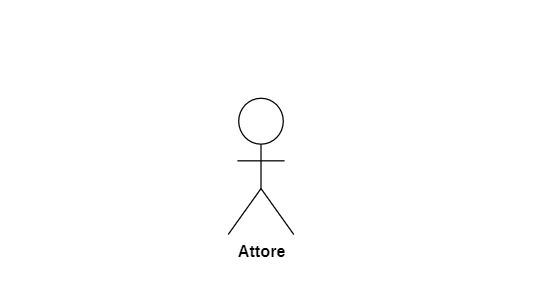
\includegraphics[width=0.7\textwidth]{../Images/NormeDiProgetto/Attore.PNG}
        \captionof{figure}{Rappresentazione Attore}
    \end{minipage}

    \vspace{0.4cm}

    \item \textbf{Casi d'Uso} 
    
    I casi d'uso identificano le diverse funzionalità offerte dal \textit{sistema}\textsubscript{\textit{G}} con cui l'attore può interagire. \\
    Ogni caso d'uso viene rappresentato tramite una forma ovale contenente un \textit{ID}\textsubscript{\textit{G}} ed un titolo esplicativo.
    \begin{minipage}[H]{\linewidth}
        \centering
        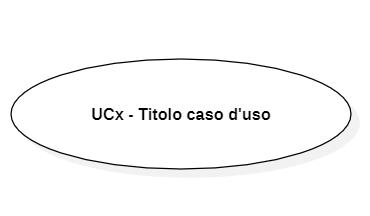
\includegraphics[width=0.6\textwidth]{../Images/NormeDiProgetto/UC.PNG}
        \captionof{figure}{Rappresentazione caso d'uso}
    \end{minipage}
    \pagebreak

    \item \textbf{Sottocasi d'uso}
    
    Un sottocaso d'uso rappresenta una versione più dettagliata di un caso d'uso più generico, offrendo un livello di dettaglio più approfondito sulle funzionalità o sui particolari scenari di utilizzo rispetto al caso d'uso principale.

    \vspace{0.2cm}
    
    \begin{minipage}[H]{\linewidth}
        \centering
        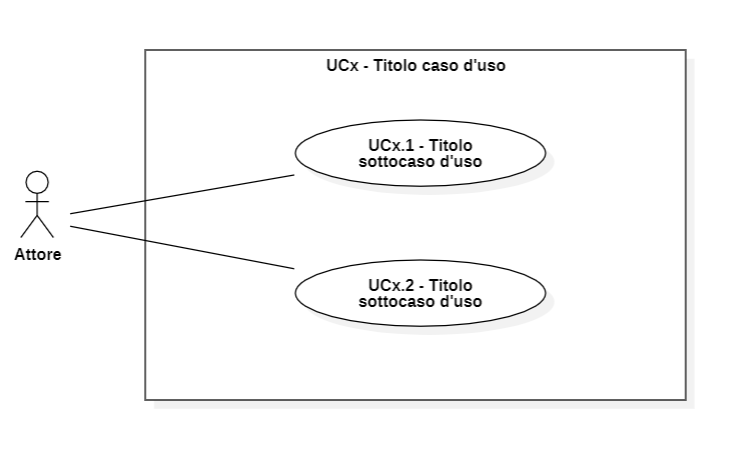
\includegraphics[width=0.6\textwidth]{../Images/NormeDiProgetto/SottocasoD'Uso.PNG}
        \captionof{figure}{Rappresentazione sottocaso d'uso}
    \end{minipage}

    \vspace{0.4cm}

    \item \textbf{Sistema}
    
    Il \textit{sistema}\textsubscript{\textit{G}} viene rappresentato da un rettangolo e viene identificato con un titolo. All'interno del \textit{sistema}\textsubscript{\textit{G}} saranno collocati i casi d'uso, mentre al suo esterno gli attori.
    \begin{minipage}[H]{\linewidth}
        \centering
        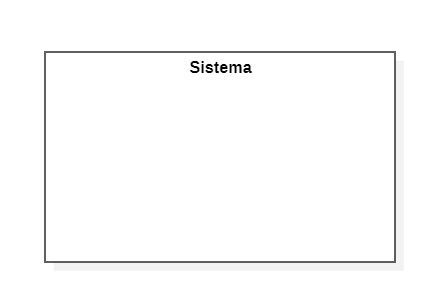
\includegraphics[width=0.6\textwidth]{../Images/NormeDiProgetto/Sistema.PNG}
        \captionof{figure}{Rappresentazione sistema}
    \end{minipage}
    \pagebreak

    \item \textbf{Relazioni tra Attori e Casi d'Uso}
    
    \begin{itemize}
        \item \textbf{Associazione} \\
        Le linee di associazione collegano gli attori ai casi d'uso corrispondenti, indicando quali attori sono coinvolti in una particolare interazione. Più precisamente, una linea di associazione collega un attore a un caso d'uso quando quell'attore è coinvolto nell'interazione descritta dal caso d'uso stesso. Questo legame rappresenta visivamente il ruolo dell'attore nell'utilizzo o nell'avvio di una funzione specifica offerta dal \textit{sistema}\textsubscript{\textit{G}}.
        
        \begin{minipage}[H]{\linewidth}
            \centering
            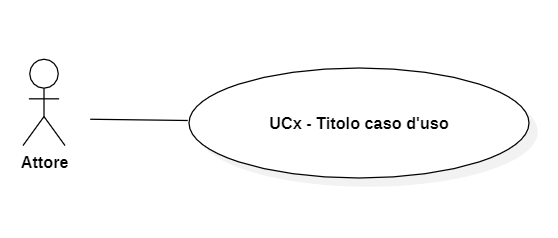
\includegraphics[width=0.6\textwidth]{../Images/NormeDiProgetto/Associazione.PNG}
            \captionof{figure}{Rappresentazione associazione}
        \end{minipage}
    \end{itemize}

    \vspace{0.4cm}

    \item \textbf{Relazioni tra attori}
    \begin{itemize}
        \item \textbf{Generalizzazione tra attori} \\
        La generalizzazione tra attori rappresenta una relazione di ereditarietà, dove un attore specializzato (figlio) eredita comportamenti e caratteristiche da un attore base (genitore).

        Questo aiuta a organizzare gerarchicamente gli attori coinvolti nell'interazione con il \textit{sistema}\textsubscript{\textit{G}} nei diagrammi dei casi d'uso. \\
        Viene rappresentata con una linea solida e una freccia vuota che parte dall'attore figlio e arriva all'attore padre.

        \begin{minipage}[H]{\linewidth}
            \centering
            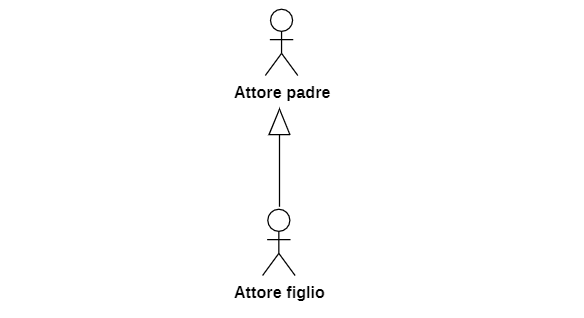
\includegraphics[width=0.6\textwidth]{../Images/NormeDiProgetto/GeneralizzazioneAttori.PNG}
            \captionof{figure}{Rappresentazione generalizzazione tra attori}
        \end{minipage}
    \end{itemize}
    
    \item \textbf{Relazioni tra casi d'uso} \\
    \begin{itemize}
        \item \textbf{Inclusione} \\
        La relazione di inclusione indica che un caso d'uso (detto "includente") include l'esecuzione di un altro caso d'uso (detto "incluso").

        In pratica, quando un attore interagisce con il caso d'uso includente, il caso d'uso incluso viene eseguito come parte integrante del primo. Questo è utile per favorire il riutilizzo e per evitare duplicazione in diversi casi d'uso.

        La relazione di inclusione viene rappresentata da una freccia tratteggiata che collega il caso d'uso incluso al caso d'uso che lo include.

        Esempio: Supponiamo che per un applicazione e-commerce ci sia un caso d'uso "Conferma ordine". Questo caso d'uso può includere il caso d'uso "Visualizza carrello". Dopo la conferma dell'ordine, l'utente viene automaticamente reindirizzato alla visualizzazione del carrello al fine di ottenere una panoramica completa dei contenuti dell'ordine.

        \vspace{1cm}

        \begin{minipage}[H]{\linewidth}
            \centering
            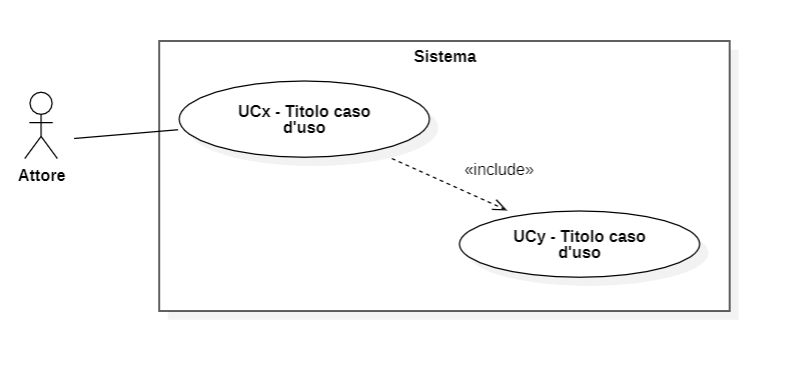
\includegraphics[width=0.7\textwidth]{../Images/NormeDiProgetto/Inclusione.PNG}
            \captionof{figure}{Rappresentazione inclusione}
        \end{minipage}

        \pagebreak

        \item \textbf{Estensione} \\
        La relazione di estensione indica che un caso d'uso (detto "estendente") può estendere il comportamento di un altro caso d'uso (detto "esteso") in determinate circostanze. In altre parole, l'esecuzione del caso d'uso estendente può essere estesa o arricchita dal caso d'uso esteso al verificarsi di determinate condizioni.

        La relazione di estensione è rappresentata da una freccia tratteggiata che collega il caso d'uso estendente al caso d'uso esteso.
        
        Esempio: Considera un caso d'uso "Visualizzazione errore di autenticazione". Questo caso d'uso potrebbe estendere il caso d'uso "Autenticazione" se durante la fase di autenticazione si inseriscono username e/o password non validi. In questo modo, l'estensione permette di gestire situazioni alternative senza ingombrare lo scenario principale di un caso d'uso e permettendo di evitare duplicazione.

        \vspace{0.6cm}
        
        \begin{minipage}[H]{\linewidth}
            \centering
            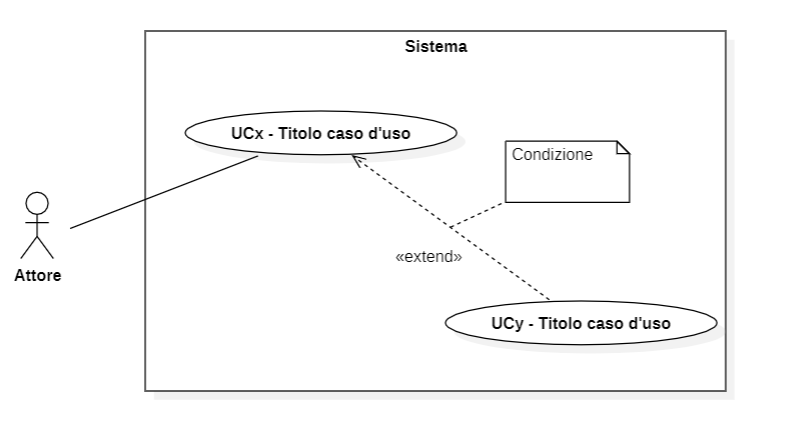
\includegraphics[width=0.6\textwidth]{../Images/NormeDiProgetto/Estensione.PNG}
            \captionof{figure}{Rappresentazione estensione}
        \end{minipage}
        \pagebreak

        \item \textbf{Generalizzazione casi d'uso} \\
        La generalizzazione nei diagrammi dei casi d'uso rappresenta una relazione di ereditarietà tra casi d'uso, indicando che un caso d'uso più specifico eredita il comportamento da un caso d'uso più generico.

        Questa relazione è simboleggiata da una linea con una freccia vuota che punta dal caso d'uso più specifico al caso d'uso più generico.

        \vspace{0.6cm}

        \begin{minipage}[H]{\linewidth}
            \centering
            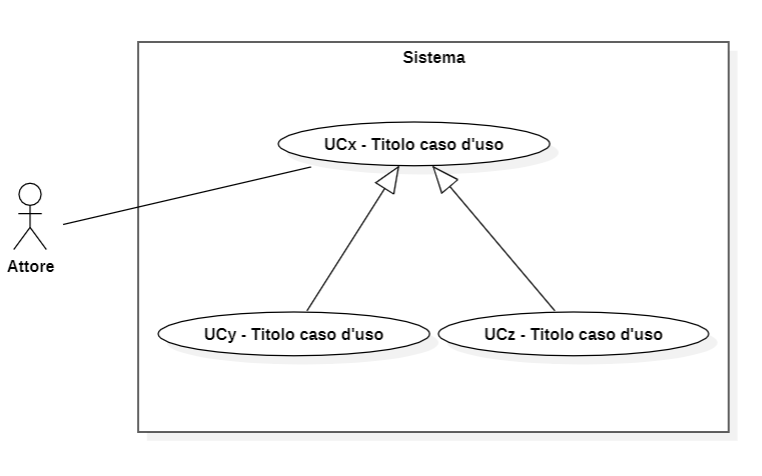
\includegraphics[width=0.6\textwidth]{../Images/NormeDiProgetto/GeneralizzazioneUC.PNG}
            \captionof{figure}{Rappresentazione generalizzazione}
        \end{minipage}
    \end{itemize}
\end{itemize}

\vspace{0.2cm}

\paragraph{Requisiti}
I requisiti di un prodotto \textit{software}\textsubscript{\textit{G}} sono specifiche dettagliate e documentate che delineano le funzionalità, le prestazioni, i vincoli e altri aspetti critici che il \textit{software}\textsubscript{\textit{G}} deve soddisfare. Questi requisiti fungono da guida per lo sviluppo, il testing e la valutazione del prodotto, assicurando che risponda alle esigenze degli utenti e agli obiettivi del progetto.

Includono:

\begin{itemize}
    \item \textbf{Requisiti funzionali:} descrivono le funzionalità che il \textit{software}\textsubscript{\textit{G}} deve avere.
    \item \textbf{Requisiti non funzionali:} definiscono principalmente criteri di prestazione, qualità, sicurezza e vincoli del \textit{sistema}\textsubscript{\textit{G}}, ovvero caratteristiche che non riguardano direttamente le funzionalità specifiche del \textit{software}\textsubscript{\textit{G}}.
\end{itemize}

Una precisa definizione dei requisiti è fondamentale: devono risultare inequivocabili e rispondere pienamente alle attese del cliente o del \textit{proponente}\textsubscript{\textit{G}}.
\pagebreak

Ogni requisito è costituito da:
\begin{enumerate}
    \item \textbf{Identificativo} nel formato:\\
    \begin{center}
        \textbf{R [Abbreviazione tipologia requisito] [Codice]}
    \end{center}
    con:
    \begin{itemize}
        \item \textbf{Abbreviazione tipologia requisito:}
            \begin{itemize}
                \item \textbf{RF:} requisito funzionale;
                \item \textbf{RQ:} requisito qualitativo;
                \item \textbf{RV:} requisito di vincolo.
            \end{itemize}
        \item \textbf{Codice:} Identificativo progressivo all'interno della tipologia di requisito.
    \end{itemize}
    \item \textbf{Importanza:}
          \begin{itemize}
              \item \textbf{Obbligatorio:} irrinunciabile per qualcuno degli \textit{stakeholder}\textsubscript{\textit{G}};
              \item \textbf{Desiderabile:} non strettamente necessario ma a valore aggiunto;
              \item \textbf{Opzionale:} relativamente utile o contrattabile più avanti nel tempo.
          \end{itemize}
    \item \textbf{Descrizione:} narrazione chiara e dettagliata che fornisce una spiegazione completa del comportamento o della caratteristica che il \textit{software}\textsubscript{\textit{G}} deve possedere;
    \item \textbf{Fonte:} fonte del requisito (ex. Capitolato, Verbale interno/esterno);
    \item \textbf{Casi d'uso:} elenco casi d'uso associati.
\end{enumerate}

\vspace{0.3cm}

\paragraph{Metriche}
Le metriche nell'\textit{analisi dei requisiti}\textsubscript{\textit{G}} sono strumenti utilizzati per valutare, misurare e gestire diversi aspetti dei requisiti di un \textit{sistema}\textsubscript{\textit{G}} o di un progetto. Queste metriche aiutano a garantire che i requisiti siano completi, corretti, coerenti e comprensibili.

\vspace{0.2cm}

\begin{table}[H]
    \centering
    \begin{tabular}{|C{3cm}|L{4cm}|C{3cm}|}
    \hline
    \textbf{Metrica} & \centering{\textbf{Nome}} & \textbf{Riferimento} \\
    \hline \hline
    M18PROS & Percentuale di Requisiti Obbligatori Soddisfatti & \hyperlink{item:M18PROS}{M18PROS} \\
    M19PRDS & Percentuale di Requisiti Desiderabili Soddisfatti & \hyperlink{item:M19PRDS}{M19PRDS} \\
    M20PRPS & Percentuale di Requisiti Opzionali & \hyperlink{item:M20PRPS}{M20PRPS} \\
    \hline
    \end{tabular}
    \caption{Metriche relative all'attività di analisi dei requisiti}
\end{table}

\paragraph{Strumenti}
\begin{itemize}
    \item \textbf{StarUML:} applicazione \textit{software}\textsubscript{\textit{G}} utilizzata dal team per la realizzazione dei diagrammi dei casi d'uso.
\end{itemize}

\subsubsection{Progettazione}

\paragraph{Descrizione}
Lo scopo primario dell'\textit{attività}\textsubscript{\textit{G}} di progettazione consiste nell'identificare una soluzione realizzativa ottimale che soddisfi appieno le esigenze di tutti gli \textit{stakeholder}\textsubscript{\textit{G}}, considerando i requisiti e le risorse disponibili.

\vspace{0.2cm}

La progettazione risponde alla domanda chiave: 'Qual è il modo migliore per realizzare ciò di cui c'è bisogno?'.

\vspace{0.2cm}

È cruciale definire l'\textit{architettura}\textsubscript{\textit{G}} del prodotto prima di avviare la fase di codifica, perseguendo correttezza per costruzione piuttosto che correttezza per correzione. Questo approccio permette di gestire in modo efficiente la complessità del prodotto, garantendo una struttura robusta e coesa durante l'intero processo di sviluppo.

\paragraph{Obiettivi}
L'obiettivo principale è quindi quello di assicurare il soddisfacimento dei requisiti attraverso un \textit{sistema}\textsubscript{\textit{G}} di qualità delineato dall'\textit{architettura}\textsubscript{\textit{G}} del prodotto.

Questo comporta:
\begin{itemize}
    \item Identificare parti componibili conformi ai requisiti, dotate di specifiche chiare e coese, sviluppandole con risorse sostenibili e costi contenuti;
    \item Organizzare il \textit{sistema}\textsubscript{\textit{G}} in modo da agevolare adattamenti futuri;
    \item Gestire la complessità del \textit{sistema}\textsubscript{\textit{G}} attraverso una progettazione dettagliata, suddividendo il \textit{sistema}\textsubscript{\textit{G}} in unità architetturali per semplificare la codifica di ciascuna parte, rendendola facilmente gestibile, veloce e verificabile.
\end{itemize}
Inizialmente, il team di progettazione condurrà un'analisi approfondita per selezionare con attenzione le tecnologie più adatte, valutandone attentamente i punti di forza, le debolezze ed eventuali criticità.

\vspace{0.2cm}

Una volta individuate le tecnologie appropriate, si procede allo sviluppo di un'\textit{architettura}\textsubscript{\textit{G}} di alto livello per comprendere e delineare la struttura generale del prodotto, costituendo così una base di partenza per la realizzazione del \textit{PoC}\textsubscript{\textit{G}}.
Questa \textit{architettura}\textsubscript{\textit{G}} fornisce una visione panoramica del \textit{sistema}\textsubscript{\textit{G}}, identificando i principali componenti, i flussi di dati e le interazioni tra di essi. Si presterà particolare attenzione a rendere il \textit{sistema}\textsubscript{\textit{G}} flessibile e adatto a potenziali modifiche future.

\vspace{0.2cm}

Successivamente, si avvierà lo sviluppo di un Proof of Concept (\textit{PoC}\textsubscript{\textit{G}}), parte fondamentale della Technology Baseline, per valutare le decisioni prese riguardo all'\textit{architettura}\textsubscript{\textit{G}} e alle tecnologie adottate, nonché per verificarne l'aderenza agli obiettivi e alle specifiche del progetto. 

\vspace{0.2cm}

In seguito allo sviluppo e ad un'attenta analisi del \textit{POC}\textsubscript{\textit{G}}, si procederà con iterazioni aggiuntive, apportando miglioramenti, aggiustamenti e aggiunte, fino a giungere a un design completo. Questo design sarà fondamentale per lo sviluppo dell'\textit{MVP}\textsubscript{\textit{G}} (Minimum Viable Product), che costituirà una versione essenziale e funzionale del prodotto e che sarà parte della Product Baseline.

\paragraph{Documentazione}

\vspace{0.2cm}

\textbf{Specifica tecnica}

Il documento descrive in modo approfondito il design definitivo del prodotto e fornisce istruzioni precise agli sviluppatori, guidandoli nella corretta implementazione della soluzione \textit{software}\textsubscript{\textit{G}} secondo i requisiti e le specifiche indicate. Ciò permette di ridurre la complessità e le ambiguità nel processo di sviluppo del \textit{software}\textsubscript{\textit{G}}, contribuendo a garantire che il prodotto finale sia allineato alle aspettative del cliente e funzioni in modo ottimale.

Questo documento comprende diversi elementi cruciali: 
\begin{itemize}
    \item \textbf{Tecnologie utilizzate}: specifica le tecnologie e le \textit{librerie}\textsubscript{\textit{G}} di terze parti integrate nel \textit{sistema}\textsubscript{\textit{G}};
    \item \textbf{Architettura logica}: definisce i componenti, i ruoli, le connessioni e le interazioni nel \textit{sistema}\textsubscript{\textit{G}};
    \item \textbf{Architettura di deployment}: indica come le componenti architetturali vengono allocate e distribuite nel \textit{sistema}\textsubscript{\textit{G}} in esecuzione;
    \item \textbf{Pattern architetturali e design pattern}: descrive i design \textit{pattern}\textsubscript{\textit{G}} architetturali adottati e quelli influenzati dalle tecnologie utilizzate;
    \item \textbf{Vincoli e linee guida}: include restrizioni e regole da seguire durante lo sviluppo;
    \item \textbf{Procedure di testing e validazione}: indica i \textit{processi}\textsubscript{\textit{G}} per testare e verificare che il \textit{software}\textsubscript{\textit{G}} soddisfi i requisiti specificati;
    \item \textbf{Requisiti tecnici}: specifica in dettaglio i requisiti prestazionali, di sicurezza, di scalabilità e di compatibilità con determinate piattaforme che il \textit{software}\textsubscript{\textit{G}} deve soddisfare.
\end{itemize}

\paragraph{Qualità dell'architettura}
\begin{itemize}
    \item \textbf{Sufficienza}: l'\textit{architettura}\textsubscript{\textit{G}} soddisfa i requisiti funzionali e non funzionali definiti per il \textit{software}\textsubscript{\textit{G}}, senza sovradimensionamento o sottodimensionamento;
    \item \textbf{Comprensibilità}: la chiarezza e la facilità con cui è possibile comprendere l'\textit{architettura}\textsubscript{\textit{G}} \textit{software}\textsubscript{\textit{G}}, rendendo agevole per gli sviluppatori e gli \textit{stakeholder}\textsubscript{\textit{G}} capire come funziona il \textit{sistema}\textsubscript{\textit{G}};
    \item \textbf{Modularità}: l'\textit{architettura}\textsubscript{\textit{G}} è suddivisa in moduli o componenti chiaramente definiti, consentendo la separazione delle responsabilità e facilitando la manutenzione, l'aggiornamento e lo sviluppo parallelo;
    \item \textbf{Robustezza}: la capacità del \textit{software}\textsubscript{\textit{G}} di gestire situazioni anomale o errate senza interruzioni gravi o perdite di dati, mantenendo un funzionamento accettabile;
    \item \textbf{Flessibilità}: la facilità con cui il \textit{sistema}\textsubscript{\textit{G}} può essere adattato o esteso per soddisfare nuovi requisiti o cambiamenti senza richiedere modifiche radicali o strutturali;
    \item \textbf{Riusabilità}: la capacità di riutilizzare parti del \textit{software}\textsubscript{\textit{G}} in contesti diversi, riducendo lo sforzo di sviluppo e migliorando l'efficienza;
    \item \textbf{Efficienza}: il \textit{software}\textsubscript{\textit{G}} utilizza in modo ottimale le risorse disponibili, come memoria e CPU, per eseguire le sue funzioni nel minor tempo possibile;
    \item \textbf{Affidabilità}: la capacità del \textit{software}\textsubscript{\textit{G}} di svolgere correttamente le sue funzioni in modo coerente e prevedibile nel tempo;
    \item \textbf{Disponibilità}: il \textit{software}\textsubscript{\textit{G}} è accessibile e operativo quando richiesto, riducendo al minimo i tempi di inattività non pianificati;
    \item \textbf{Sicurezza rispetto a malfunzionamenti (Safety)}: la prevenzione di danni fisici o danni a persone o beni a causa di malfunzionamenti del \textit{software}\textsubscript{\textit{G}};
    \item \textbf{Sicurezza rispetto a intrusioni (Security)}: la protezione del \textit{software}\textsubscript{\textit{G}} da accessi non autorizzati, manipolazioni e intrusioni esterne;
    \item \textbf{Semplicità}: la capacità di mantenere l'\textit{architettura}\textsubscript{\textit{G}} \textit{software}\textsubscript{\textit{G}} il più semplice possibile senza compromettere la funzionalità o l'efficacia;
    \item \textbf{Incapsulazione}: il nascondere dei dettagli implementativi all'esterno di un componente, consentendo l'accesso solo attraverso un'interfaccia definita;
    \item \textbf{Coesione}: la misura in cui i componenti all'interno di un modulo o un'unità funzionano insieme per un obiettivo comune senza essere eccessivamente interdipendenti;
    \item \textbf{Basso accoppiamento}: il grado di dipendenza tra i diversi moduli o componenti del \textit{software}\textsubscript{\textit{G}}, cercando di minimizzare le interazioni o le dipendenze tra di essi per migliorare la manutenibilità e la flessibilità del \textit{sistema}\textsubscript{\textit{G}}.
\end{itemize}

\paragraph{Diagrammi UML}
Vantaggi:
\begin{itemize}
    \item \textbf{Chiarezza nella comunicazione}: rendono più comprensibili e chiari i concetti tecnici ai team e agli \textit{stakeholder}\textsubscript{\textit{G}};
    \item \textbf{Standardizzazione}: offrono un linguaggio comune per la documentazione e la comprensione dei sistemi \textit{software}\textsubscript{\textit{G}};
    \item \textbf{Analisi e progettazione visiva}: aiutano a identificare errori e lacune nel progetto prima dell'implementazione;
    \item \textbf{Modellazione e simulazione}: consentono la creazione di modelli predittivi, riducendo rischi e costi durante lo sviluppo;
    \item \textbf{Facilitano la manutenzione}: semplificano la comprensione della struttura del \textit{software}\textsubscript{\textit{G}}, agevolando le operazioni di manutenzione;
    \item \textbf{Riducono errori di progettazione}: aiutano a individuare problemi prima dell'implementazione, riducendo correzioni costose;
    \item \textbf{Supportano la documentazione}: offrono una guida visiva per comprendere il \textit{sistema}\textsubscript{\textit{G}}, inclusa nella documentazione del progetto.
\end{itemize}

A supporto dell'\textit{attività}\textsubscript{\textit{G}} di progettazione verranno utlizzati i \textbf{Diagrammi delle classi}. \\

\paragraph*{Diagrammi delle classi}
Ciascun diagramma delle classi rappresenta le proprietà e le relazioni tra le varie componenti di un \textit{sistema}\textsubscript{\textit{G}}, offrendo una prospettiva statica e non a run time.

\vspace{0.2cm}

Le classi sono rappresentate graficamente sotto forma di rettangoli divisi in tre sezioni:

\begin{enumerate}
    \item \textbf{Nome della classe}: identificativo della classe. \\
    È rappresentato in grassetto seguendo la convenzione PascalCase e deve esplicitare chiaramente la responsabilità della classe. Se la classe è astratta, il nome viene scritto in corsivo;
    \pagebreak
    \item \textbf{Attributi}: ogni elemento sarà presentato in una riga separata, secondo il seguente formato: \\
    \begin{center}\texttt{Visibilità Nome: Tipo [Molteplicità] = Valore/i di Default}\end{center}
    \begin{itemize}
        \item \textbf{Visibilità}: precede obbligatoriamente ogni attributo e rappresenta uno dei seguenti indicatori:
        \begin{itemize}
            \item $-$ : visibilità privata;
            \item $+$ : visibilità pubblica;
            \item $\#$ : visibilità protetta;
            \item $\sim$ : visibilità di package.
        \end{itemize}
        \item \textbf{Nome}: rappresenta univocamente l'attributo. Dev'essere rappresentativo dell'attributo e deve seguire la notazione \texttt{nomeAttributo: tipo}. \\
        Qualora l'attributo fosse di tipo costante, allora il nome verrà scritto interamente in maiuscolo \texttt{NOMEATTRIBUTO: tipo};
        \item \textbf{Molteplicità}: nel caso di una sequenza di elementi, come liste o array, la sua lunghezza può essere specificata con la sintassi \texttt{tipoAttributo[molteplicità]}. \\
        Se la sequenza contiene un numero di elementi non conosciuto a priori, verrà adottata la sintassi \texttt{tipoAttributo[*]}. \\
        Nel caso di un singolo elemento, la sua dichiarazione è opzionale;
        \item \textbf{Default}: ogni attributo può essere dichiarato con un valore di default.
    \end{itemize}
    
    \item \textbf{Firme dei metodi}: descrivono il comportamento delle classi individuate. Ogni metodo occuperà una riga e seguiranno il formato: \\
    \begin{center} \texttt{Visibilità Nome (Parametri Formali): Tipo di Ritorno} \end{center}
    \begin{itemize}
        \item \textbf{Visibilità}: segue la convenzione definita per gli attributi;
        \item \textbf{Nome}: rappresenta l'identificativo univoco del metodo e descrive in modo esplicito il suo obiettivo, seguendo la notazione \textit{PascalCase};
        \item \textbf{Parametri formali}: il loro numero varia da $0$ a $n$ e sono separati tramite la virgola. Ogni parametro seguirà la notazione e le convenzioni definite per gli attributi;
        \item \textbf{Tipo di ritorno}: determina il tipo che verrà ritornato dal metodo.
    \end{itemize}
\end{enumerate}

\pagebreak

\paragraph*{Convenzioni sui metodi}
\begin{itemize}
    \item I metodi getter, setter e i costruttori non vengono inclusi fra i metodi;
    \item I metodi astratti sono scritti in corsivo; 
    \item I metodi statici sono sottolineati;
    \item L'assenza di attributi o metodi in una classe, determina una visualizzazione di campi vuoti nel diagramma delle classi.
\end{itemize}

\paragraph*{Relazioni tra le classi}
I diagrammi delle classi sono collegati tra loro mediante frecce che delineano le rispettive relazioni di dipendenza. \\
Qui di seguito, saranno delineate le rappresentazioni mediante frecce per le diverse relazioni: \\
\begin{itemize}
    \item \textbf{Dipendenza}\\
    Se la classe A utilizza servizi, metodi o membri forniti dalla classe B, si dice che la classe A dipende dalla classe B e tale relazione viene rappresentata con una freccia tratteggiata dalla classe A alla classe B. \\
    La relazione di dipendenza indica il minor grado di accoppiamento tra due classi: un cambiamento nella classe B può influenzare la classe A, ma non viceversa.
    \begin{figure}[H]
        \centering
        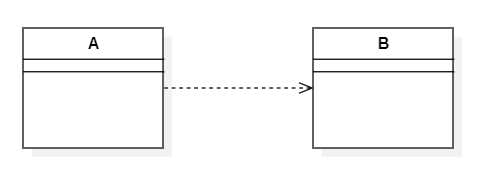
\includegraphics[width=0.6\textwidth]{../Images/NormeDiProgetto/ClassDiagram_Dipendenza.PNG}
        \caption{Diagramma delle classi di una relazione di Dipendenza.}
    \end{figure}
    \vspace{0.4cm}
    
    \item \textbf{Associazione}

    L'associazione tra due classi viene rappresentata tramite una linea continua e orientata. Questa connessione indica che la classe A contiene campi o istanze della classe B. \\
    Le molteplicità di occorrenza possono essere espresse tramite valori posizionati agli estremi della freccia:
    \begin{itemize}
        \item $\mathbf{0...1}$: A può possedere 0 o 1 istanza di B;
        \item $\mathbf{0...*}$: A può possedere 0 o più istanze di B;
        \item $\mathbf{1}$:  A possiede esattamente un'istanza di B (in questo caso non è necessario specificare la molteplicità);
        \item $\mathbf{*}$: A possiede più istanze di B;
        \item $\mathbf{n}$: A possiede esattamente n istanze di B.
    \end{itemize}
    \begin{figure}[H]
        \centering
        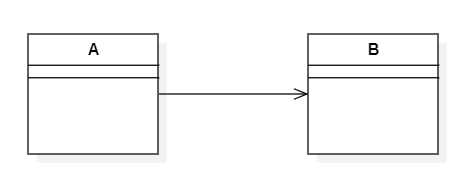
\includegraphics[width=0.6\textwidth]{../Images/NormeDiProgetto/ClassDiagram_Associazione.PNG}
        \caption{Diagramma delle classi di una relazione di Associazione.}
    \end{figure}

    \vspace{0.4cm}
    
    \item \textbf{Aggregazione}
    
    Rappresentata con una freccia a diamante vuota.

    Indica una relazione "parte di" (part of) in cui una classe è composta da diverse parti (altre classi), ma le parti possono esistere anche indipendentemente dalla classe principale. Nella figura la classe B è parte della classa A.
    \begin{figure}[H]
        \centering
        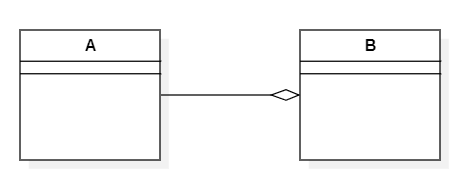
\includegraphics[width=0.6\textwidth]{../Images/NormeDiProgetto/ClassDiagram_Aggregazione.PNG}
        \caption{Diagramma delle classi di una relazione di Aggregazione.}
    \end{figure}
    \pagebreak    

    \item \textbf{Composizione}
    
    Rappresentata con una freccia a diamante piena. È simile all'aggregazione, ma le parti (altre classi) sono strettamente dipendenti dalla classe principale e non possono esistere indipendentemente. \\
    Nella figura la classe B è parte della classe A ed esiste solo come parte di A.
    \begin{figure}[H]
        \centering
        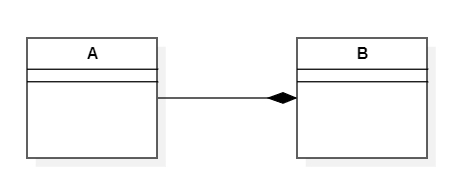
\includegraphics[width=0.6\textwidth]{../Images/NormeDiProgetto/ClassDiagram_Composizione.PNG}
        \caption{Diagramma delle classi di una relazione di Composizione.}
    \end{figure}

    \vspace{0.4cm}

    \item \textbf{Generalizzazione} 
    
    Rappresentata con una freccia continua vuota. Rappresenta la relazione "is a" (è un) tra una classe genitore (superclasse) e una classe figlia (sottoclasse). La classe figlia eredita attributi e comportamenti dalla classe genitore. \\
    Equivale all'ereditarietà nei linguaggi di programmazione. \\
    Le proprietà della superclasse non si riportano nel diagramma della sottoclasse, a meno di override.
    \begin{figure}[H]
        \centering
        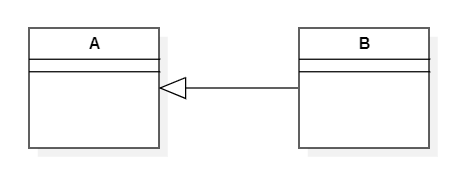
\includegraphics[width=0.6\textwidth]{../Images/NormeDiProgetto/ClassDiagram_Generalizzazione.PNG}
        \caption{Diagramma delle classi di una relazione di Generalizzazione.}
    \end{figure}

    \pagebreak
    
    \item \textbf{Interface Realization}
    
    La relazione di "interface realization" indica che una classe fornisce l'implementazione dei metodi definiti in un'interfaccia specifica. Questa relazione è importante quando si desidera mostrare come una classe concreta soddisfi i requisiti di un'interfaccia specifica definendo e implementando i suoi metodi.

    Nella figura l'interfaccia A, rappresentata tramite un cerchio, viene implementata dalla classe B e questa relazione viene rappresentata graficamente con una linea da B ad A.
    \begin{figure}[H]
        \centering
        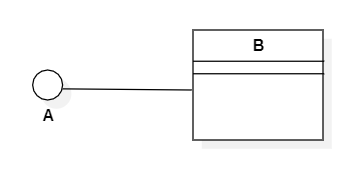
\includegraphics[width=0.6\textwidth]{../Images/NormeDiProgetto/InterfaceRealization.PNG}
        \caption{Diagramma delle classi di una relazione di Interface Realization.}
    \end{figure}
\end{itemize}

\paragraph{Design Pattern}
I design \textit{pattern}\textsubscript{\textit{G}} costituiscono una risposta consolidata a problemi di progettazione che si presentano ciclicamente in determinati contesti. Questi modelli offrono un approccio di progettazione riusabile, garantendo qualità nella soluzione ed una rapida implementazione.

L'adozione di un design \textit{pattern}\textsubscript{\textit{G}} avviene soprattutto quando una soluzione si è dimostrata efficace in un contesto specifico.

\vspace{0.2cm}

Solitamente vengono fornite guide dettagliate sull'applicazione dei \textit{pattern}\textsubscript{\textit{G}}, delineando il loro utilizzo ottimale.
Ogni design \textit{pattern}\textsubscript{\textit{G}} deve essere accompagnato da una rappresentazione grafica illustrativa del suo funzionamento, da una spiegazione testuale della sua logica e da una descrizione della sua utilità all'interno dell'\textit{architettura}\textsubscript{\textit{G}} complessiva. 

\vspace{0.2cm}

Questa documentazione svolge un ruolo chiave nel favorire una comprensione approfondita dell'\textit{integrazione}\textsubscript{\textit{G}} del design \textit{pattern}\textsubscript{\textit{G}} nell'\textit{architettura}\textsubscript{\textit{G}} generale e nella prevenzione di errori di progettazione.

\paragraph{Test}
Nell'ambito del processo di sviluppo, il testing riveste un ruolo fondamentale nell'assicurare la qualità del prodotto finale. Durante questa fase, si delineano i requisiti di testing, si definiscono i casi di \textit{test}\textsubscript{\textit{G}} e i criteri di accettazione, fungendo da strumenti per valutare il \textit{software}\textsubscript{\textit{G}}.

\vspace{0.2cm}

Il suo obiettivo principale è individuare e risolvere eventuali problemi o errori presenti nel \textit{software}\textsubscript{\textit{G}} prima del rilascio del prodotto finale. In aggiunta, il processo di testing è essenziale per garantire che il \textit{software}\textsubscript{\textit{G}} soddisfi le specifiche e le aspettative del cliente.

\vspace{0.2cm}

I progettisti avranno il completo controllo di questa \textit{attività}\textsubscript{\textit{G}}, compresa la definizione dei \textit{test}\textsubscript{\textit{G}} da eseguire. Inoltre, nella sezione \ref{subsubsec:Testing}, si può trovare una descrizione dettagliata delle varie tipologie di \textit{test}\textsubscript{\textit{G}} e della terminologia da adottare, offrendo così un'ulteriore chiarezza su questa fase critica del processo di sviluppo del \textit{software}\textsubscript{\textit{G}}.

\paragraph{Metriche}
\begin{table}[H]
    \centering
    \begin{tabular}{|C{3cm}|C{4cm}|C{3cm}|}
    \hline
    \textbf{Metrica} & \centering{\textbf{Nome}} & \textbf{Riferimento} \\
    \hline \hline
    M25ATC & Accoppiamento tra classi (ATC) & \hyperlink{item:M25ATC}{M25ATC}\\
    M30PG & Profondità delle Gerarchie (PG) &  \hyperlink{item:M30PG}{M30PG}\\
    M31TMR & Tempo Medio di Risposta (TMR) & \hyperlink{item:M31TMR}{M31TMR}\\
    M32FU & Facilità di Utilizzo (FU) & \hyperlink{item:M32FU}{M32FU}\\
    M33TA & Tempo di Apprendimento (TA) & \hyperlink{item:M33TA}{M33TA}\\
    M34VBS & Versioni dei Browser Supportate (VBS) & \hyperlink{item:M34VBS}{M34VBS}\\
    \hline
    \end{tabular}
    \caption{Metriche relative all'attività di progettazione}
\end{table}

\paragraph{Strumenti}
\begin{itemize}
    \item \textbf{StarUML:} applicazione \textit{software}\textsubscript{\textit{G}} utilizzata per la realizzazione dei diagrammi delle classi.
\end{itemize}

\subsubsection{Codifica}
\paragraph{Descrizione}
L'\textit{attività}\textsubscript{\textit{G}} di codifica è affidata al ruolo del programmatore e rappresenta il momento cruciale in cui le funzionalità richieste dal \textit{proponente}\textsubscript{\textit{G}} prendono forma. \\
Durante questa fase, le idee e i concetti delineati dai progettisti vengono tradotti in codice, creando istruzioni e procedure che i calcolatori possono eseguire. \\
I programmatori devono rispettare scrupolosamente le linee guida e le norme stabilite per garantire che il codice sia in linea con le specifiche stabilite e che traduca in modo accurato le concezioni iniziali dei progettisti.
\paragraph{Obiettivi}
La codifica è finalizzata alla creazione di un prodotto \textit{software}\textsubscript{\textit{G}} in linea con le richieste del \textit{committente}\textsubscript{\textit{G}} e conforme agli accordi stipulati.\\
Il rigoroso rispetto delle norme garantisce la creazione di codice di alta qualità, facilitando la manutenzione, l'estensione e la verifica del \textit{software}\textsubscript{\textit{G}}, contribuendo costantemente al miglioramento della sua qualità complessiva.
\paragraph{Norme di codifica}
Le seguenti norme sono state formalizzate prendendo spunto dal libro "Clean Code" di Robert C. Martin.

\begin{itemize}
    \item \textbf{Nomi significativi}: usare nomi che riflettano il significato e lo scopo delle variabili, funzioni e classi. Evitare abbreviazioni ambigue;
    \item \textbf{Indentazioni e formattazione consistente}: l'utilizzo di un tab per ciascun livello di annidamento è fondamentale per assicurare una struttura coerente del codice, migliorandone la comprensione e agevolandone la gestione;
    \item \textbf{Lunghezza dei metodi}: la lunghezza ottimale dei metodi può variare a seconda del contesto e delle best practices di programmazione. Tuttavia, in generale, molti esperti consigliano che i metodi siano brevi e focalizzati su una singola responsabilità. Un principio comune è quello espresso da Robert C. Martin nel suo libro "Clean Code", che suggerisce che i metodi dovrebbero essere idealmente lunghi quanto basta per svolgere una singola operazione e non più lungo di quanto si possa visualizzare senza dover scorrere la pagina. 
    
    Questo favorisce:
    \begin{itemize}
        \item \textbf{Chiarezza};
        \item \textbf{Manutenibilità};
        \item \textbf{Comprensibilità};
        \item \textbf{Testabilità:} metodi più brevi sono più facili da testare in isolamento, il che favorisce l'implementazione di \textit{test}\textsubscript{\textit{G}} di unità efficaci;
        \item \textbf{Conformità ai principi SOLID:} la brevità dei metodi è spesso correlata al principio Single Responsibility Principle (\textit{SRP}\textsubscript{\textit{G}}) dei principi \textit{SOLID}\textsubscript{\textit{G}}, il che favorisce la costruzione di codice più modulare e coeso.
    \end{itemize} 
    \item \textbf{Lunghezza righe di codice}: mantenere le righe di codice entro i 80-120 caratteri permette una migliore leggibilità del codice su schermi di diverse dimensioni e facilita la visualizzazione di più file affiancati. Inoltre, limitare la lunghezza delle righe può incoraggiare la scrittura di codice più chiaro e modulare;
    \item \textbf{Commenti} \\
    Evitare commenti superflui e non necessari: l'obiettivo è scrivere il codice in modo chiaro e autoesplicativo, riducendo la dipendenza da commenti esplicativi.
\end{itemize}

\vspace{0.1cm}

\paragraph{Strumenti}
\begin{itemize}
    \item \textbf{Visual Studio Code:} IDE utilizzato dal team di sviluppo per la codifica del prodotto \textit{software}\textsubscript{\textit{G}}.
\end{itemize}

\vspace{0.1cm}

\paragraph{Metriche}
\begin{table}[H]
    \centering
    \begin{tabular}{|C{3cm}|C{4cm}|C{3cm}|}
    \hline
    \textbf{Metrica} & \centering{\textbf{Nome}} & \textbf{Riferimento} \\
    \hline \hline
    M15SC & Statement Coverage (\textit{MSC}\textsubscript{\textit{G}}) &  \hyperlink{item:M15SC}{M15SC} \\
    M16BC & Branch Coverage (MBC) &  \hyperlink{item:M16BC}{M16BC} \\
    M17CNC & CoNdition Coverage (CNC) &  \hyperlink{item:M17CNC}{M17CNC} \\
    M26MCCM & Complessità Ciclomatica per Metodo (\textit{MCCM}\textsubscript{\textit{G}}) &  \hyperlink{item:M26MCCM}{M26MCCM} \\
    M27PM & Parametri per metodo (PM) & \hyperlink{item:M27PM}{M27PM} \\
    M28APC & Attributi per classe (APC) & \hyperlink{item:M28APC}{M28APC} \\
    M29LCM & Linee di codice per metodo (LCM) & \hyperlink{item:M29LCM}{M29LCM} \\ 
    \hline
    \end{tabular}
    \caption{Metriche relative all'attività di codifica}
\end{table}

\pagebreak

\subsubsection{Configurazione dell'ambiente di esecuzione}

\paragraph{Docker}

La scrittura dei file \textit{Docker}\textsubscript{\textit{G}} è considerata parte del processo di sviluppo del \textit{software}\textsubscript{\textit{G}}. \\
Le regole e le \textit{best practice}\textsubscript{\textit{G}} di codifica per i file \textit{Docker}\textsubscript{\textit{G}} sono fondamentali per garantire la creazione, la gestione e la distribuzione efficace dei \textit{container}\textsubscript{\textit{G}}:
\begin{itemize}
    \item \textbf{Chiarezza e Coerenza:}
    \begin{itemize}
        \item Utilizzare nomi descrittivi per le immagini e i \textit{container}\textsubscript{\textit{G}}.
        \item Mantenere una struttura coerente e consistente per assicurare un'organizzazione uniforme all'interno dei file \textit{Docker}\textsubscript{\textit{G}}.
    \end{itemize}

\item \textbf{Versionamento:}
    \begin{itemize}
        \item Specificare sempre la versione dell'immagine di base (base image) per garantire la riproducibilità.
        \item Evitare di utilizzare tag "latest" per immagini di produzione.
    \end{itemize}

\item \textbf{Minimizzazione degli strati (Layering):}
    \begin{itemize}
        \item Ridurre il numero di istruzioni nell'esecuzione del \textit{Dockerfile}\textsubscript{\textit{G}} per minimizzare gli strati dell'immagine.
        \item Raggruppare le istruzioni correlate per sfruttare la cache \textit{Docker}\textsubscript{\textit{G}}.
    \end{itemize}

\item \textbf{Sicurezza:}
    \begin{itemize}
        \item Utilizzare immagini ufficiali o verificate.
        \item Evitare di eseguire \textit{processi}\textsubscript{\textit{G}} \textit{Docker}\textsubscript{\textit{G}} con privilegi elevati quando possibile.
        \item Usare ARG per parametrizzare informazioni sensibili.
    \end{itemize}

\item \textbf{Ottimizzazione delle risorse:}
    \begin{itemize}
        \item Limitare l'uso di risorse all'interno dei \textit{container}\textsubscript{\textit{G}} (CPU, memoria, etc.).
        \item Usare immagini leggere e ottimizzate per la produzione.
    \end{itemize}

\item \textbf{Gestione delle variabili d'ambiente:}
    \begin{itemize}
        \item Usare variabili d'ambiente per configurazioni dinamiche.
        \item Fornire valori predefiniti opportuni per le variabili d'ambiente.
    \end{itemize}
\pagebreak

\item \textbf{Logging e monitoraggio:}
    \begin{itemize}
        \item Configurare i \textit{container}\textsubscript{\textit{G}} per registrare i \textit{log}\textsubscript{\textit{G}} in modo efficace.
        \item Integrare strumenti di monitoraggio, se necessario.
    \end{itemize}

\item \textbf{Pulizia e riduzione delle dimensioni:}
    \begin{itemize}
        \item Pulire i pacchetti temporanei e le risorse non necessarie dopo l'installazione delle dipendenze.
        \item Ridurre le dimensioni delle immagini utilizzando \textit{multi-stage builds}\textsubscript{\textit{G}}.
    \end{itemize}

\item \textbf{Documentazione:}
    \begin{itemize}
        \item Aggiungere commenti nel \textit{Dockerfile}\textsubscript{\textit{G}} per spiegare le decisioni di progettazione.
        \item Fornire una documentazione chiara su come utilizzare e configurare il \textit{container}\textsubscript{\textit{G}}.
    \end{itemize}

\item \textbf{Testing:}
    \begin{itemize}
        \item Implementare \textit{test}\textsubscript{\textit{G}} automatizzati per il \textit{Dockerfile}\textsubscript{\textit{G}} e i \textit{container}\textsubscript{\textit{G}}, se possibile.
    \end{itemize}
\end{itemize}
\paragraph{Strumenti}
\begin{itemize}
    \item \textbf{Visual Studio Code:} IDE utilizzato dal team di sviluppo per la codifica dei file \textit{Docker}\textsubscript{\textit{G}}.
    \item \textbf{Docker:} \textit{piattaforma}\textsubscript{\textit{G}} di virtualizzazione leggera che permette di creare e gestire applicazioni in contenitori \textit{software}\textsubscript{\textit{G}}, fornendo un ambiente portatile, scalabile ed efficiente per lo sviluppo, il testing e la distribuzione delle applicazioni.
\end{itemize}
